\chapter{Oficina física}\label{S:tema_1}
Este tema define los requisitos teóricos de la construcción de una oficina en remoto, contrastada con dos setups, uno mi habitación de estudio reconvertida en oficina durante la pandemia de 2020-21 véase \ref{S:setup_pandemia} y el diseño implementación y uso de “mi oficina-virtual” durante 2022-23. Los requisitos se catalogan en 7 categorías (véase anexo \ref{S:requisitos}), \textbf{mínimo, adecuado y óptimo} respecto a la calidad del requisito; y \textbf{básico, profesional, profesional pro y business} en relación a el coste.


\section{Requisitos}
En este apartado se define la base adecuada para una oficina en casa o también útil como base elemental de oficina para una startup tecnológica.

\subsection{Elementos físicos}
Entendemos como mínimo indispensable un pc o laptop para realizar la tarea, sin embargo esto es “la falacia estudiantil”. Realizar un trabajo profesional de manera continuada ( 8 horas), sin interrupciones y concentrado no debe llevarse a cabo en espacios públicos o familiares. Las malas condiciones posturales así como climatización o la inestabilidad de servicios claves como internet degradan la calidad final del trabajo\cite{c_postura} y contribuyen psicológicamente en una actitud negativa del trabajador\cite{c_postura_covid}.

 Está claro que un elemento implícito es el espacio de trabajo, una habitación, un cubículo, un coworking, su principal función es permitir instalar en el el setup informático quien es el verdadero centro de la oficina. Pero otros aspectos como tener una iluminación y ventilación adecuada, así como facilitar la organización de apuntes, herramientas o periféricos necesarios durante la jornada laboral son tan importantes como el propio setup.

Finalmente se ha definido espacialmente, el doble del tamaño de un cubículo de las bibliotecas de UPC como el espacio adecuado y una habitación dedicada como óptima. 

\subsection{Setup informático}
En el anexo \ref{S:setup_informatico} mencionan las principales corrientes en la selección y montaje de un setup. En mi opinión y como conclusión se recomienda encarecidamente un setup basado en laptop, aunque puede utilizarse un pc o mini pc. Es requisito indispensable un monitor extendido de 24’-27’, aunque se recomienda el uso de dos pantallas (\ref{S:pantallas}). El uso de periféricos tales como ratón/teclado, auriculares con micrófono, todos ellos conectados a través de un elemento centralizador de interconexión de pantallas, pc/laptop.

Respecto al hardware existe una evolución histórica\cite{c_guia_hardware}, cuellos de botella y estrategias a la hora de planificar la compra y mantenimiento de los diferentes componentes del  hardware, como resumen en el punto \ref{S:hardware_recursos}, detalla las estrategias a utilizar en la selección de hardware sin la comprensión del mismo.

 En base a las estrategias de selección de hardware, en el contexto actual (2023) la prioridad es la utilización de las nuevas plataformas RAM DDR5 enlazadas con las últimas series de procesadores AMD Ryzen o Intel; ram adecuada de 16 GB, 32 GB óptimo, discos duros SSD o NVMe de 512 GB - 1 TB.

Focalizando en modalidades 8 cores (adecuado), es decir, procesadores Ryzen 5/7, o Intel i5/i7 que como configuración final puede presupuestarse entre 900-1200€ + mantenimiento 100-150€ en 2026.

Pero siguiendo una estrategia ‘b’, pueden conseguirse ofertas significativas para obtener un hardware bastante equivalente basado en ddr4 en el rango 500-700€ y 100€ de mantenimiento en 2025, y planificar un reemplazo por un hardware nuevo de  600-800€ en 2027.

Por último existe una extensión de la estrategia ‘b’ basada en mini pc, la cual aunque degrada la movilidad y el mantenimiento, permite obtener un hardware sin GPU equivalente por 250-400€ y un mantenimiento 100-150€ en 2025.

 Respecto a las tarjetas gráficas deben ser adecuadas a las necesidades del trabajador. Un programador puede usar gráfica cpu-embedded, pero actividades gráficas o renderizado requieren de GPU dedicadas. En caso de optar por GPU integradas, los procesadores AMD Ryzen tienen una clara ventaja sobre Intel tanto en performance, como en calidad-precio.

Para un mayor detalle así como entender la selección y mantenimiento del setup recomendamos encarecidamente la lectura del anexo \ref{S:anexo_B} o guía externa  para hardware \cite{c_guia_hardware}.

\subsection{Conectividad}
Toda infraestructura asumida en el espacio de trabajo, son los llamados abastecimientos auxiliares (véase anexo \ref{S:abastecimientos_auxiliares}), ya que sin ellos no es posible realizar el trabajo o en algunos casos degrada tanto la eficacia como la comodidad del trabajador.

Internet o conectividad es el requisito indispensable, ya que una oficina puede existir pero no ser en remoto. Otra cosa es definir las propiedades de la conexión, como solución general el requisito de una conexión con un mínimo de \textbf{15 / 5 Mbps (down/up)}, con \textbf{delays} no mayores a \textbf{75 ms} y tasas baja de \textbf{jamming 30 ms}, es decir, un servicio de ADSL céntrico, cable coaxial, conectividad 3G/4G/5G urbana o fibra estándar cumplen o superan las características requeridas.

 De especial interés el análisis comparativo de la tabla \ref{T:comp_conexion_tech} que cataloga aquellas tecnologías no aptas, problemáticas o poco apropiadas por calidad precio, como son Wimax, internet por satélite o ADSL en zonas rurales.

\section{Tabla de Requisitos}
 En la tabla \ref{T:tabla_requisitos} resume los diferentes requisitos necesarios de una oficina física para teletrabajar. Aquellos que comienzan con “\textbf{+}” hace referencia a extender en anterior requisito con más elementos. Las categorías o elementos marcados indicados con “\textbf{*}” son de uso obligatorio. Véase un acoplamiento generalizado entre prestaciones y costes, que no representa la realidad de mercado, sino una tendencia intencionada para buscar las mejores prestaciones en base a un precio límite. 
\begin{table}[!htbp]
\begin{center}
   
    \caption{Tabla de requisitos físicos, oficina.}
\resizebox{15cm}{!} {
 \label{T:tabla_requisitos}
    \begin{tabular}{|p{3.5cm}|p{3cm}|p{3cm}|p{3cm}|p{3cm}|}    
    \hline    
        ~ & {\bf Mínimo - Básico} &  {\bf Adecuado - Procesional} & {\bf Óptimo - Profe.Pro} & {\bf Óptimo - Business}  \\ \hline
        
        Espacio de trabajo* & cubículo UPC & escritorio personal  & habitación / coworking & despacho dedicado \\ \hline
        
        Iluminación* & luz blanca oficina & +luz natural & +regular luz natural & +regular luz artificial  \\ \hline
        
        Ventilación* & manual & automático & aclimatado & aclimatado con renovación \\ \hline
        
        Hardware Base* & pc-torre & mini-pc laptop & laptop especializado & hardware sobre dimensionado o exclusivo \\ \hline
                
        CPU* cores & 4 cores 2-3 años & 8 cores 1-2 años & 8-16 cores 1-2 años & 12/16/32 cores  < 1 año  \\ \hline
        
        RAM* & ddr4 8-12 GB & ddr4 16 GB ddr5 8-16 GB & ddr4 32 GB ddr5 16-32 GB & ddr5 32 GB \\ \hline

        Disco Duro* & SSD 256 GB 100 - 200 MB/s  & SSD 512 GB - 1000 GB 400-600 MB/s & SSD mayor 1 TB 600-1000 MB/s & NVMe 1-2 TB 1000 - 7000 MB/s \\ \hline

        Pantallas* & x1 21'-24‘, HD & x2 21’-24', HD-FHD & x2 27’ FHD-2K & x2-x3 27’-34’ 2K-4K \\ \hline

        Periféricos & webcam micro* auriculares* ratón* & HD cam* HD micro Auriculares HF ratón-teclado inalámbrico*  & +cam bloqueable +auriculares con cancelación de ruido +pad táctil o bolígrafo táctil  & +cam HD cancelación de ruido y micrófono estéreo +software eliminación de sonido externos \\ \hline

        Elemento centralizador & - & Cable VGA/HDMI Hub usb & dock-station* extender usb-vga-hdmi  & hub-station usb-c  \\ \hline
        
        Elemento de seguridad & - & lector de tarjeta con pin & lector de huellas & llave usb con cierre de lector huellas  \\ \hline
        
        Elemento opcionales & alfombrilla ratón pomodoro & +reposamuñecas +reposapiés +monitor elevado & +monitores ajustables +ratón ergonómico & +VR \\ \hline
        
        Conectividad* & ADSL / 3G urbano & ADSL2 / VDSL / 4G / cable coaxial Fibra 100 MB/s  & Fibra >300 MB/s 5G & StarLink \\ \hline
        
        Extras & almacenaje estanterías y cajones & impresora / escaner / telefono ip & kit electronica soldador impresora 3D pizarra & projector alexa / google home / sensoring hub \\ \hline
        
        Seguridad & cajonera con llave & +ip cam & +habitación con llave & +sensores de puerta o presencia \\ \hline
       
    \end{tabular}
}
\end{center}
\end{table}

La gran mayoría de los requisitos de un setup eficiente para un uso profesional deben de estar enmarcados en opciones “\textbf{adecuadas-profesionales}” u “\textbf{óptimo - profesional-pro}”. En concreto el caso de estudio de este trabajo se centra en un enfoque “óptimo” siempre que el precio sea “profesional”, o degradado a “adecuado” por la mejora de relación calidad-coste.


 \section{Diseño Práctico}

 En este apartado se plantea un problema real, “crear un espacio y acondicionarlo” para permitir la instalación de un setup real asumiendo la solución teórica de los requisitos anteriores.

\subsection{Circunstancias e histórico}

En el anexo \ref{S:circunstancias}, se especifican las condiciones generales, pre pandémica, durante la pandemia y post pandemia. Podemos resumirlas en “siempre he contado con una habitación dedicada como despacho compartida con mi pareja”, dicha habitación tenía un uso estudiantil así como para hobbies. Varios elementos, tales como pantalla, conexión de internet o espacio dedicado, hacían inviable su uso real como lugar de teletrabajo. 

La remodelación (véase \ref{S:setup_pandemia}) y mejora durante y post pandemia la convirtió en un lugar apto para teletrabajar (monopolizado por mi), sin embargo dicha remodelación estaba dirigida a una función más familiar (habitación para niños).  En 2022 se descarta completamente el uso de la habitación puesto que para finales de ese año se espera la incorporación de un nuevo miembro a la familia. Las nuevas circunstancias (véase \ref{F:setup_bebe}) obligan a la búsqueda de un espacio adecuado y reconstrucción completa de la habitación de teletrabajo, diseñada bajo los parámetros del punto 1.2 de este trabajo. Así como la planificación de una nube privada aplicable tanto a mi oficina para proyectos personales, como al trabajo de mi pareja para flexibilizar o facilitar el trabajo remoto con la nueva incorporación familiar.

\subsection{Creación de un espacio de trabajo}

En el anexo \ref{S:nueva_room} se especifican posibles soluciones espaciales, así como las circunstancias detalladas del problema. Tras evaluar las diferentes posibilidades finalmente la solución es crear un espacio de trabajo utilizando una caseta de aluminio a medida hermética.

Esta solución elimina una zona mal drenada y hundida de la terraza y que no es útil debido a una respiradero-chimenea comunitario así mismo se combina con armario de aluminio en otra zona infrautilizada para realojar aquellos elementos que ocupaban el espacio de la caseta.

Por lo tanto, debido a ser la única solución aceptable como material de construcción se usa aluminio y paneles sándwich con cámara térmica, lacados en blanco del mismo tipo que los utilizados por la comunidad de vecinos para la separación entre terrazas, apropiadamente anclados a muro, paredes y apropiadamente herméticos con silicona, especialmente suelos.

\subsection{Dimensiones y distribución}

El acceso a la caseta, así como la iluminación natural, se realizan mediante una puerta corrediza y una ventana acristalada también corredera, típicas de cerramientos de aluminio.

Con el objetivo de maximizar la capacidad, y el movimiento el techo será prácticamente plano, con una inclinación de 5º para drenar el agua. Por normativa comunitaria, dichas aguas deben caer a mi terraza, no se puede exponer nada diferente al panel de aluminio en los tramos de alféizar de la fachada.

Por lo tanto las dos únicas paredes útiles son las que disponen de la ventana (Sur-Oeste) y puerta (Oeste-Norte), y por consiguiente las otras dos paredes son las indicadas para almacenamiento y setup fig.\ref{F:planos_caseta}.

 Aunque no es lo mas deseado una 'iluminación natural lateral' en las pantallas, se dedujo que la predisposición más útil es un Setup en 'L'', utilizando la pared Oeste-Norte como base del setup y la ventana como base de la 'L' generando una mesa extendida para tareas manuales como soldadura, herramientas o disponer de un espacio extra y permitiendo la colocación de almacenaje en la pared norte (la más extensa).

\begin{figure}[htb]
\begin{center}
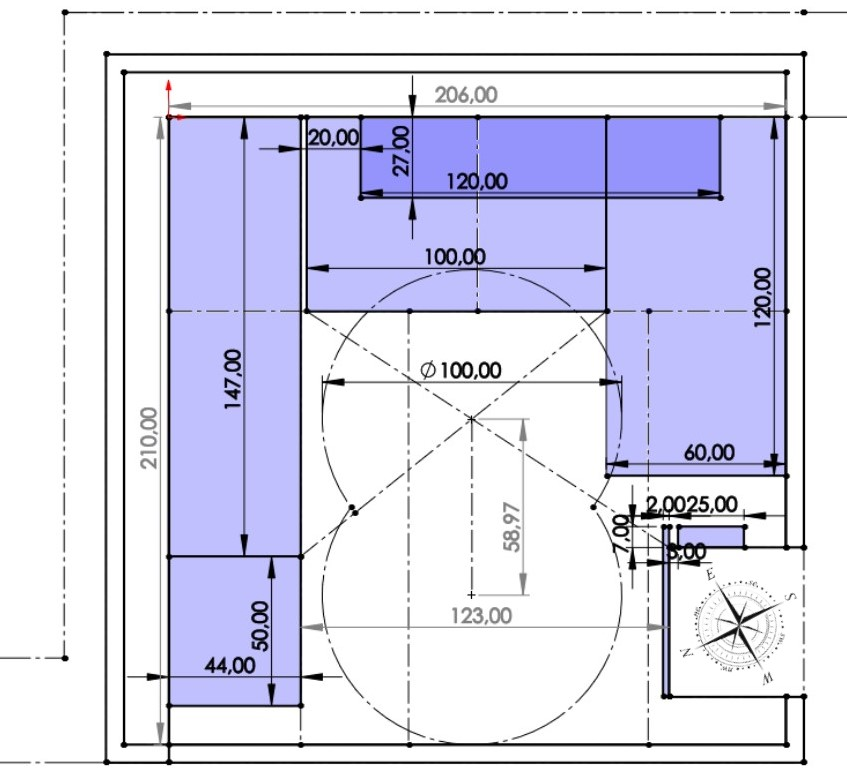
\includegraphics[width=0.9\textwidth]{./figuras/planos_caseta.jpg}
\caption{Diseño caseta, distribución mobiliario}
\label{F:planos_caseta}
\end{center}
\end{figure}

Dicha pared tiene de suelo a techo, mobiliario con cajoneras y estanterías, quedando el segundo nivel apoyado directamente sobre el medio alféizar. En el centro de la caseta se ha generado un espacio de 1-1.3 metros ideal para una silla giratoria con ruedas que accede fácilmente a toda la oficina y no entorpece el movimiento.

Por último tanto el espacio de entrada como los recovecos entre la chimenea-respiradero y el aluminio, son ampliamente funcionales debido a la puerta corredera y el uso de las pizarras este espacio es ampliamente usado como lugar de reflexión y pensamiento.

\subsection{Electricidad y Red}

La conexión eléctrica así como la conectividad se basa en una instalación nueva, extendiéndose desde la existente durante el proceso de puesta a punto previo a la instalación de armario y caseta. Con el objetivo de facilitar y separar las instalaciones, se dispondrá de un cableado de 2.5$mm^{2}$ y PIA asociado únicamente para la caseta y otro para enchufes e iluminación de terraza.

Inicialmente se contaba con un PLC de 10 Mbps que permite conexiones a través de la red eléctrica de iluminación de la terraza, sin embargo se ha instalado un cableado directo de ethernet desde la vivienda con el fin de maximizar dicha conexión a 1 Gbps.

\section{Construcción Oficina}

Este punto resume la construcción de la caseta presupuesto y tiempos aunque su detalle y pormenorizado se encuentra en el anexo \ref{S:anexo_B}.

\subsection{Acondicionamiento terraza}

Previamente a la instalación de la caseta así como del armario se realizaron un conjunto de tareas de acondicionamiento y mantenimiento previos que están descritos en anexo \ref{S:trabajos_previos} Los principales cambios fueron:

\begin{figure}[htb]
\begin{center}
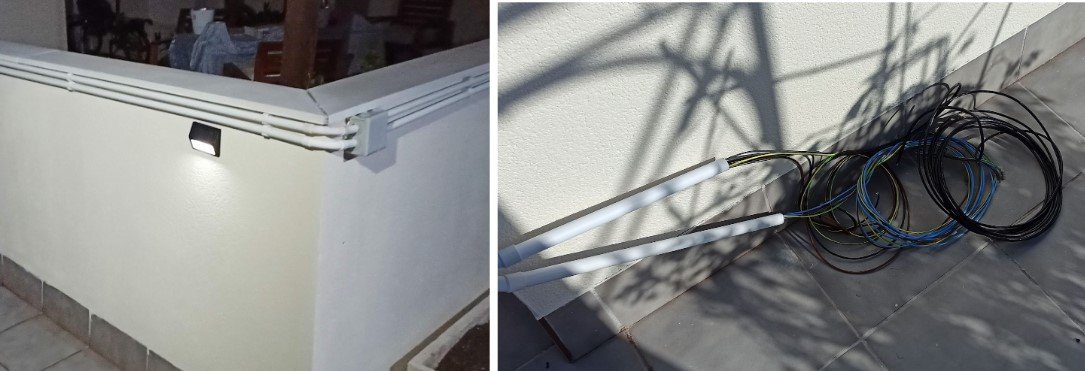
\includegraphics[width=1\textwidth]{./figuras/montaje_electrico.jpg}
\caption{Montaje eléctrico.}
\label{F:montaje_electrico}
\end{center}
\end{figure}

\begin{enumerate}
    \item Limpieza de paredes (barrido y agua a presión), alféizares con productos ácidos y suelos (con ácido clorhídrico diluido y detergente) para eliminar cal y abrir los poros.    
    \item Pintar la terraza y aplicaciones borada en juntas desgastadas entre baldosas.    
    \item Colocación de cajas y canalizaciones eléctricas en la terraza, permitiendo diferenciar, iluminación terraza, alimentación caseta y cable de red.
\end{enumerate}

\subsection{Caseta y armario}

El material de cortado así como montaje fue presupuestado y construido por una empresa local de aluminio, cerramientos, puertas y ventanas, que es la utilizada por la comunidad de vecinos para la instalación de las separaciones de medianera. En apenas 5 días la empresa encargada terminó la instalación completa de los cerramientos de aluminio, previos a la Semana Santa fig.\ref{F:estructuras_aluminio}
\begin{figure}[htb]
\begin{center}
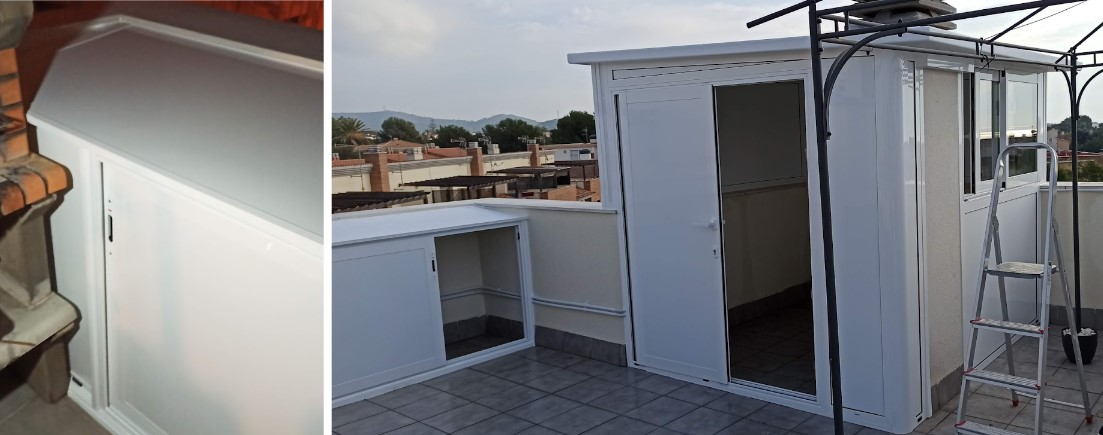
\includegraphics[width=1\textwidth]{./figuras/estructuras_aluminio.jpg}
\caption{Estructuras de aluminio.}
\label{F:estructuras_aluminio}
\end{center}
\end{figure}
En los días posteriores una vez secadas las juntas se continuó con la instalación eléctrica  tanto de armario como caseta, con puntos de luces, interruptores, enchufes y cajas internas fig.\ref{F:caseta_con_iluminacion_y_mobiliario}.
Así como un primer aislamiento de paredes y suelo con capa transparente anti-humedad previa a la colocación de mobiliario y alfombras.
\begin{figure}[htb]
\begin{center}
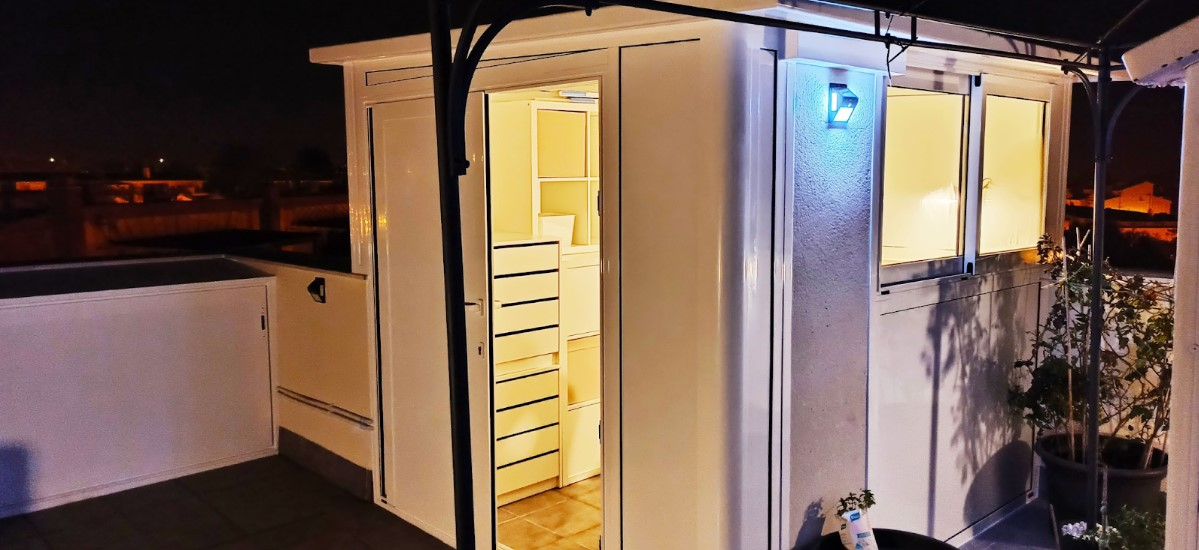
\includegraphics[width=1\textwidth]{./figuras/caseta_con_iluminacion_y_mobiliario.jpg}
\caption{Caseta iluminada}
\label{F:caseta_con_iluminacion_y_mobiliario}
\end{center}
\end{figure}
El mobiliario principalmente ikea o leroy merlin, se fundamenta en almacenamiento o estanterías apropiadamente seleccionadas para optimizar el espacio a un coste competitivo. La mesa y el elevador de pantallas son elementos estandarizados de ikea.
\begin{figure}[!htb]
\begin{center}
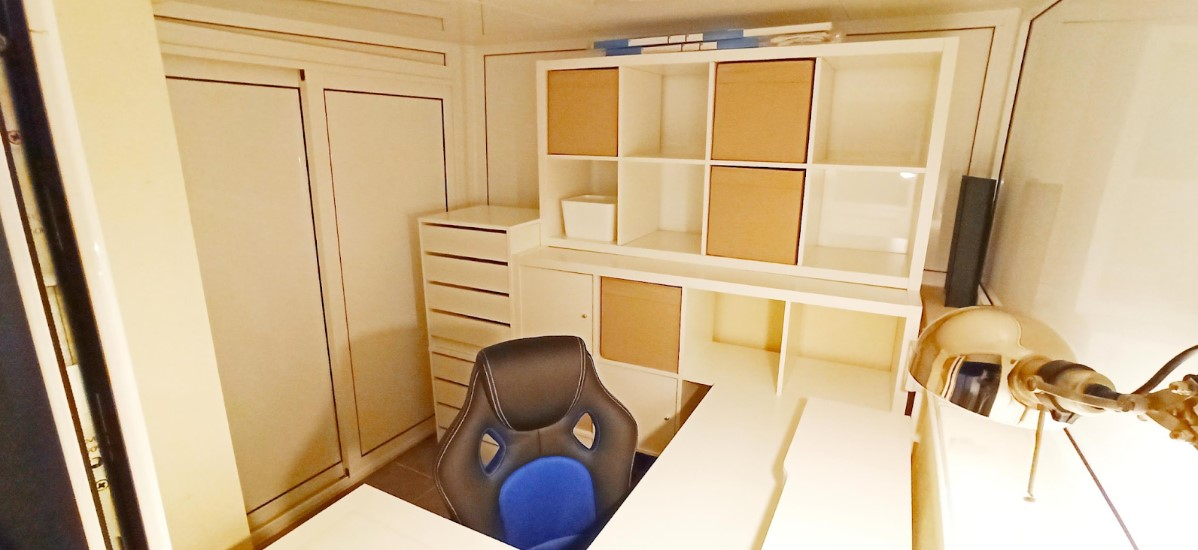
\includegraphics[width=1\textwidth]{./figuras/mobiliario_interior}
\caption{Caseta mobiliario.}
\label{F:mobiliario_interior}
\end{center}
\end{figure}

\subsection{Presupuestos planificación}

La gran mayoría de trabajos realizados a excepción de los montajes de aluminios se han realizado por este autor. Debido a ello la realización de las tareas no solo se ven limitadas por la secuencialidad de las mismas o necesidad de esperas como secado o asentamiento, sino que también se debe tener en cuenta que está mayoritariamente realizadas de viernes-domingo más días sueltos 4-6 h dedicados entre semana. Como contrapartida el coste real es “nulo” ya que no he asignado un precio real hora, pero como queda reflejado en la tabla de presupuesto con un tiempo personal muy monopolizado por la construcción.

Por ejemplo, aunque las tareas previas a la instalación de la caseta no superan los 15 días de trabajo continuado se realizaron durante Febrero-Marzo, casi 40 días laborales y 20 festivos.

\begin{figure}[!htb]
\begin{center}
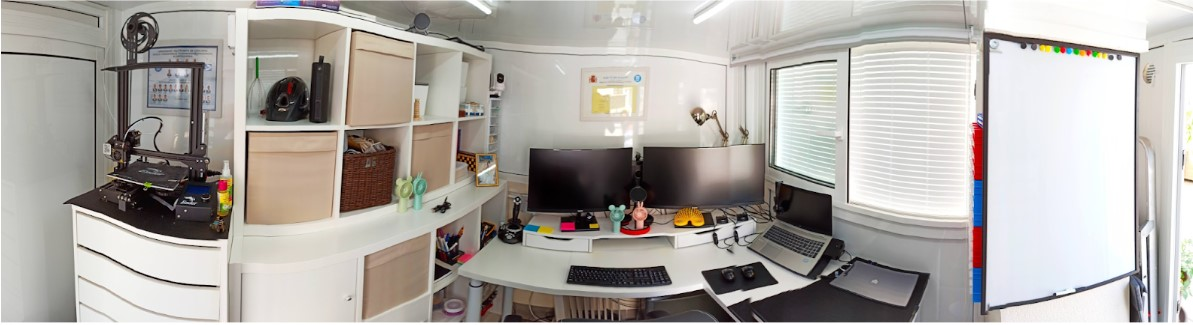
\includegraphics[width=1\textwidth]{./figuras/caseta_migrada}
\caption{Panorámica caseta migrada.}
\label{F:caseta_migrada}
\end{center}
\end{figure}
En la siguiente tabla se muestran los tiempos y costes de las tareas a realizar, que están dispuestas en orden cronológico de realización.
\begin{center}
\label{T:presupuesto}
\begin{longtable}[ht]{|p{3cm}|p{8cm}|p{1.5cm}|p{1.5cm}|}
\caption{Presupuesto Caseta Física}
    \\ \hline
    \textbf{Elemento} & \textbf{Descripción} & \textbf{Tiempo} & \textbf{Coste Material} \\ \hline
    Limpieza Alféizar & Barrer, frotar, aplicar producto limpieza especial, aclarado & 4 h & 6€ \\ \hline
    Limpieza Pared & Barrido y agua a presión & 1d & 0€ \\ \hline
    Limpieza Suelo & Barrido, fregado, limpieza con salfumán diluido & 1d & 10€ \\ \hline
    Pintar Terraza & pintado y limpieza posterior de suelo & 2d & 35€ \\ \hline
    Boradas y juntas & Aplicación y limpieza de borada en juntas. & 4d & 15€ \\ \hline
    Cajas y canalización & Colocación de cajas y canalizaciones eléctricas & 3d & 25€ \\ \hline
    Cableado Eléctrico & Pasar cableado eléctrico, interconexión de cajas y puntos de luz. & 2d & 40€ \\ \hline
    Cableado Ethernet & Adecuar cableado desde azotea comunitario, eliminar antena Wimax, pasar cableado por terraza. & 1d & 15€ \\ \hline
    Armario Aluminio Aislado & Montaje y sellado de armario por empresa. & 2d & 1500€ \\ \hline
    Caseta Aluminio & Montaje de laterales, montaje alféizar, montaje tejado, sellado. Montaje ventana y puerta. & 4d & 4500€ \\ \hline
    Luces, enchufes y tubos led & Instalación de cableado, enchufes, interruptores, cajas internas y tubos led de iluminación. & 3d & 60€ \\ \hline
    Mobiliario & Compra y montaje de mobiliario ikea & 2d & 450€ \\ \hline
    Mesa & Montaje de mesa customizada y eleva pantallas & 5h & 80€ \\ \hline
    Extras mobiliario & Separadores, protectores, cubetas ikea etc... & 1d & 60€ \\ \hline
    Pizarra & Montaje de pizarras en la chimenea-respiradero & 4h & 25€ \\ \hline
    Estore & Montaje y anclaje de estor interior difuminador de luz en ventana. & 2h & 20€ \\ \hline
    Mosquitera  & Instalar mosquitera plástica fácilmente reemplazable o reinstalable. & 1h & 4€ \\ \hline
    Persiana exterior & Compra instalación y sujeción de persiana alicantina externa de pvc. & 2d & 40€ \\ \hline
    Cámara Seguridad & IP cam con IA de reconocimiento personas con movimiento automatizado 360º & 2h & 35€ \\ \hline
    Alfombra Oficina & Alfombra robusta, oficina, con grosor extra aislante. & 2h & 80€ \\ \hline
    Mudanza & Mover el antiguo setup, herramientas, libros etc a la nueva oficina. Mover Impresora 3D, periféricos. & 3d & - \\ \hline
    Router & Router wifi para caseta y alrededores de terraza. & 1h & 25€ \\ \hline
    Switch & Switch Giga ethernet para conexiones por cable de elementos de la caseta & 1h & 20€ \\ \hline
    Google Home & Elemento interactivo de smart home dedicado a terraza y oficina & 1h & 18€ \\ \hline
    Smart things & Luces de terraza configurables (color, intensidad) accionadas por Alexa/Google assistant. Termómetro, interruptor inteligente. & 1h & 32€ \\ \hline
    Cámaras Seguridad & Cámaras de Seguridad Exterior de Terraza y Balcón, + Switch-Router que provee the conectividad a la terraza y las cámaras & 2h & 55€ \\ \hline
    Pingüino Calefactor & Pingüino, bomba calor/frió/deshumidificador para 15$m^{2}$ & 2h & 350€ \\ \hline
    ~ & ~ & ~ & ~ \\ \hline
    \textbf{Total} & ~ & \textbf{35d} & \textbf{7500€} \\ \hline
\end{longtable}
\end{center}

\subsection{Resultados de construcción}

Finalmente en mayo la caseta esta completamente terminada y 100\% funcional, siendo utilizada tanto en horario de oficina en mi trabajo, hobbies, formaciones y la elaboración de esta tesis. Así como la ejecución entre Febrero-Abril y un coste final de 7600-7800€, se puede asumir una finalización en plazo así como costes adecuados a lo planificado, no superando desvíos de 3-5\%.

\begin{figure}[htb]
\begin{center}
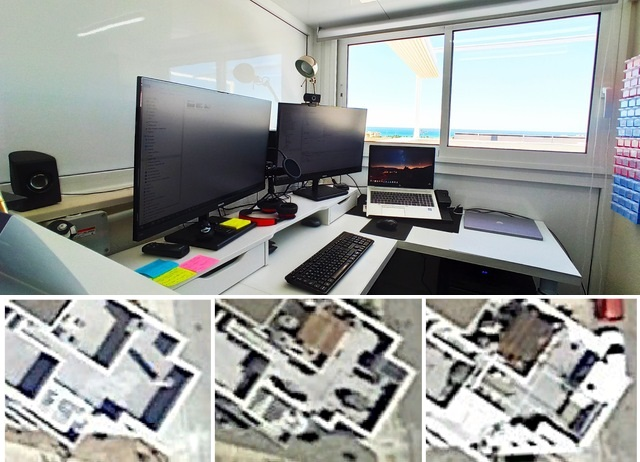
\includegraphics[width=0.9\textwidth]{./figuras/setup_mayo}
\caption{Setup en mayo, vista satélite pre pandemia, pandemia, actualidad.}
\label{F:setup_mayo}
\end{center}
\end{figure}

Véase una explicación al pormenor en el anexo B los puntos \ref{S:circunstancias} como la causa y comparativa con setups anteriores,  referentes a la construcción \ref{S:trabajos_previos}, \ref{S:estructura_aislamiento} así como otros puntos menos resaltables tales como iluminación \ref{S:iluminacion_caseta} y un conjunto no despreciable de fallos, mejoras y correcciones durante 2023 (\ref{S:cambios_2023}) que evidencian la continuación del proyecto mas allá de su desarrollo principal.

Por otra parte este proyecto de bricolaje técnico, ha servido de base para la aplicación en otros ámbitos personales del conocimiento técnico/practico adquirido, como la instalación del sistema eléctrico y solares en un almacén agrícola de mi padre; el cableado ethernet de mi casa, casa de mis padres, suegra, oficinas y en general cualquier amigo que me ha pedido ayuda con cableado ethernet y cámaras de seguridad. Así como muchos elementos del setup, y especialmente la guía\cite{c_guia_hardware} y a previsión de mantenimiento para la selección de hardware con fines profesionales a largo termino.

Finalmente como cliente y promotor de este espacio, me siento completamente satisfecho al pasar una media entre 9-13 horas de mi día a día en dicho espacio y obtener un aislamiento familiar perfecto y separación de entorno profesional y personal.
